Численное моделирование исследует поведение предложенного алгоритма для функции логистической регрессии в сравнение с классическими подходам.
Исходный код на языке Python доступен в открытом репозитории диссертации
\footnote{\url{https://github.com/NMashalov/EducationGenerativeModelApplication}}.

Ключевым параметром для анализа является соотношение изменения параметра сложности задачи $\Delta d$ к параметру роста ${\beta}$.
\begin{figure}[h]
    \centering
    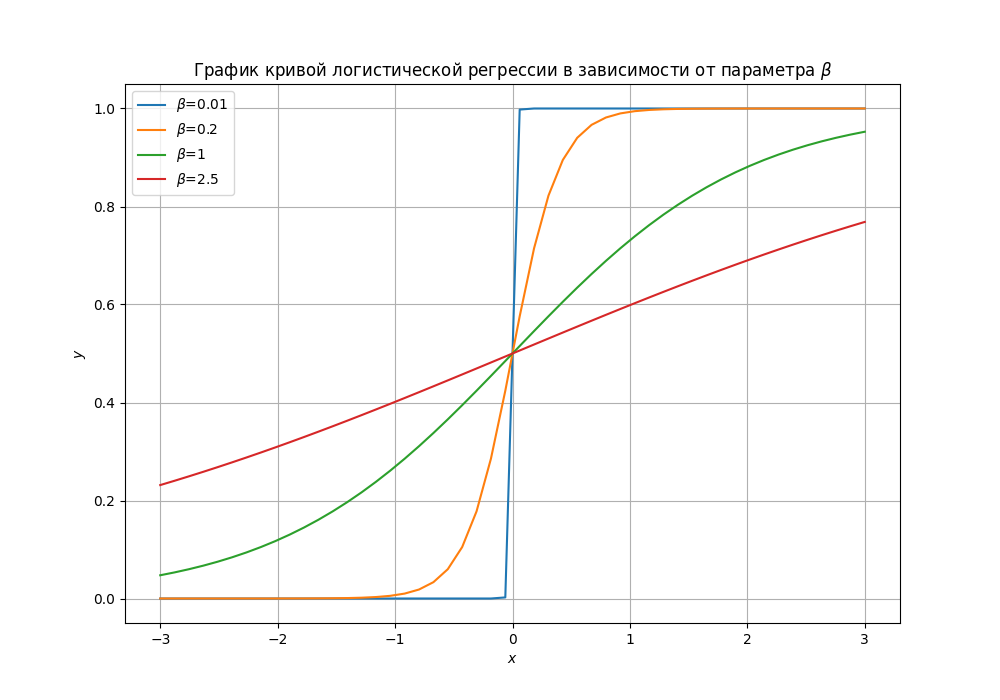
\includegraphics[width=0.8\textwidth]{assets/work/rating/logistic.png}
    \caption{Демонстрация изменения графика логистической регрессии от параметр роста}
    \label{logistic_figure}
\end{figure}
Таким образом, были исследованы две ключевые краевые постановки: \begin{enumerate}
    \item малые изменения  $\Delta d / \beta \approx 0$ 
    \item значительные изменения $\Delta d / \beta \approx 1$ 
\end{enumerate}
В каждом эксперименте сравнивалась эффективность метода с классическим алгоритмом Роббинса-Монро и его аналогом с фиксированным коэффициент $\lambda$ как в работе \cite{yazidi2020balanced}. Дополнительно изучено влияние модификации по методу Поляка скользящим средним. 

Гладкие графики траекторий получается путем визуализации среднего и перцентилей распределения. Для их численного расчета используется метод бутстрэп.
Эксперимент проводится $B >> 1$ раз, после чего статистики считаются путем расчета распределения.   

В разделе приведены ключевые графики, полный набор доступен в приложении статьи. Отметим, что при анализе сходимости число шагов $N$ определяется аналогично правилу предела.
$N$ считается шагом достижения сходимости,
если все последующие точки не выходят за границу $\epsilon$.  $\epsilon$ выбирается индивидуально из соображений статистической значимости результата. 


\subsubsection{Случай $\Delta d / \beta \approx 1$ }
Эксперимент проводился для $s(d) = \frac{1}{1+\exp(-5(d-0.6)} $ c начальной сложность $d_0 =0.2$ и целевым параметром $s^* =0.4$
\footnote{Для наглядности в таблице классический алгоритм Роббинса-Монро сокращается до сокращения "Р.-М." с указанием параметра шага.}
\begin{figure}[h]
    \centering
    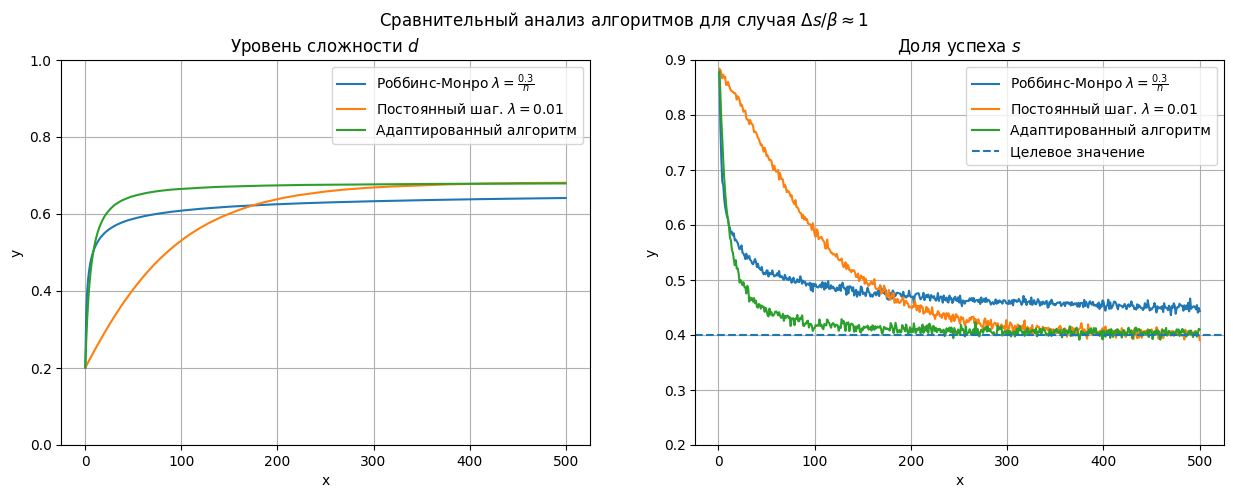
\includegraphics[width=1.0\textwidth]{assets/work/rating/1/result.png}
    \caption{Предложенный алгоритм}
    \label{exp1:algo}
\end{figure}
Отметим также чувствительность алгоритм Роббинса-Монро к параметру шага. \ref{exp1:classic}
\begin{figure}[h]
    \centering
    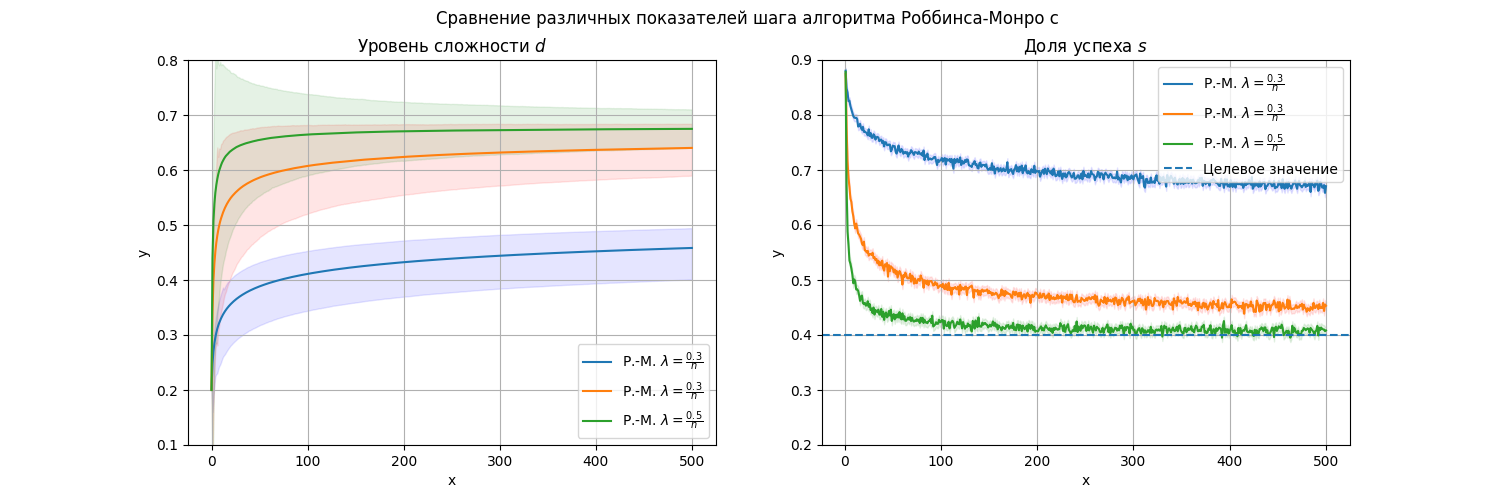
\includegraphics[width=1.0\textwidth]{assets/work/rating/1/sensitivity.png}
    \caption{Классический алгоритм Роббинса-Монро чувствителен к параметру $\lambda$}
    \label{exp1:classic}
\end{figure}
\begin{table}
    \centering
    \begin{tabular}{ ||c | c|| }
        \hline 
          \text{Название алгоритма} &  \text{Число шагов}\\
        \hline 
         \text{Постоянный} $\lambda_n = 0.01$ & $400  \pm 20$ \\  
         \text{Алгоритм Р.-М.} $\lambda_n = 0.1$ & \text{Не сошелся} \\
         \text{Алгоритм Р.-М.} $\lambda_n = 0.5$ & $250 \pm 30$ \\
         \text{Адаптированный алгоритм Р.-М.} & $200 \pm 35 $   \\
         \hline
    \end{tabular}        
    \caption{Сравнение числа шагов сходимости в постановке $\Delta d / \beta \approx 1$}
    \label{exp1:table}
\end{table}
\subsubsection{Случай $\Delta d / \beta \approx 0$ }
Эксперимент проводился для $s(d) = \frac{1}{4(d-0.6)}$ c начальной сложность $d_0 =0.2$ и целевым параметром $s=0.8$. Число раундов было выбрано минимальным для

\footnote{Для наглядности в таблице классический алгоритм Роббинса-Монро сокращается до сокращения "Р-М" с указанием параметра шага.}

\begin{figure}[h]
    \centering
    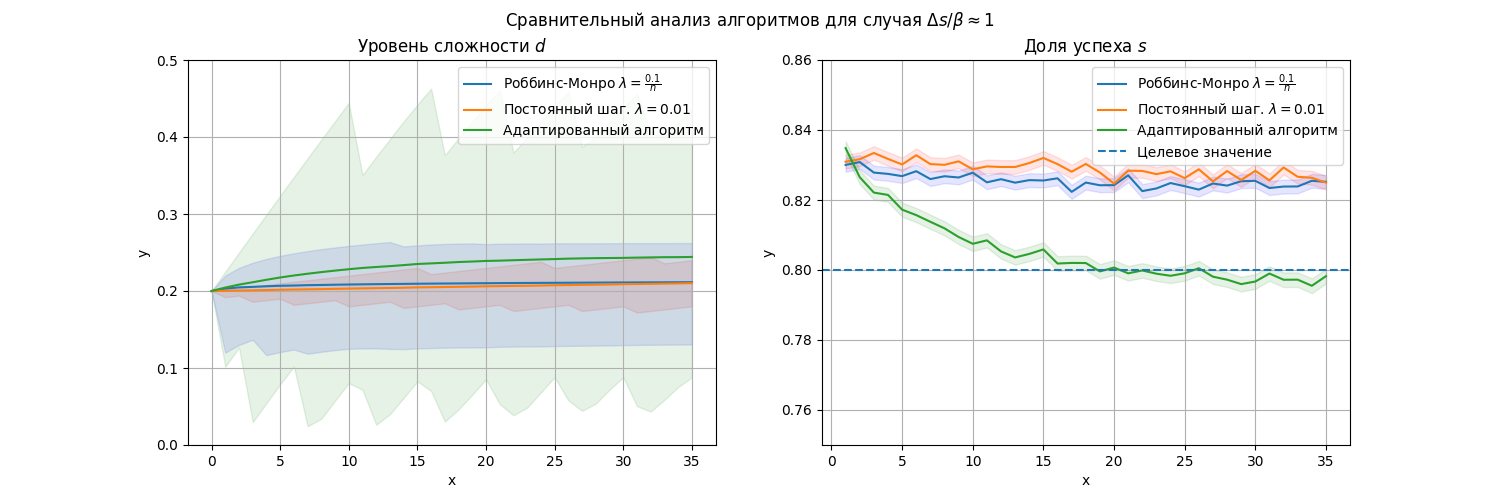
\includegraphics[width=1.0\textwidth]{assets/work/rating/2/comparison_analysis.png}
    \caption{Предложенный алгоритм имеет высокую скорость реакции $d$}
    \label{exp2:сomparison}
\end{figure}

\begin{table}
    \centering
    \begin{tabular}{ ||c | c|| }
        \hline 
        \text{Название алгоритма} &  \text{Число шагов}\\
        \hline 
        \text{Постоянный} $\lambda_n = 0.01$ & $400  \pm 20$ \\  
        \text{Алгоритм Р.-М.} $\lambda_n = 0.1$ & \text{Не сошелся} \\
        \text{Алгоритм Р.-М.} $\lambda_n = 0.5$ & $250 \pm 30$ \\
        \text{Адаптированный алгоритм  Р.-М.} & $200 \pm 35 $   \\
        \hline
    \end{tabular}
    \caption{Сравнение числа шагов сходимости в постановке $\Delta d / \beta \approx 0$}
    \label{exp2:table}
\end{table}

\subsubsection{Случай значительного отличия априорных представлений о наклоне кривой от действительного}
Рассмотрен случай, в котором $\beta$ априорная значительно отличается $\beta^*$ действительного.
\begin{figure}[h]
    \centering
    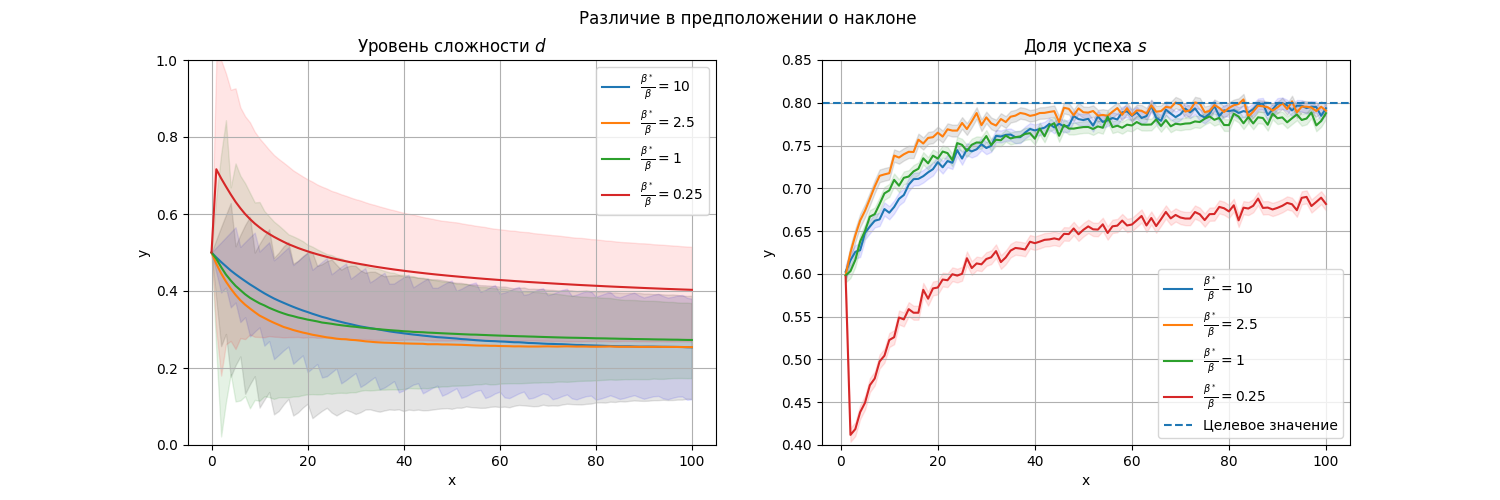
\includegraphics[width=0.9\textwidth]{assets/work/rating/3/slop_affect.png}
    \caption{Значительные различия в предположениях о наклоне логистической регрессии приводят к снижению эффективности алгоритма}
    \label{exp3:lose_effictivness}
\end{figure}
\begin{table}
    \centering
    \begin{tabular}{ ||c | c|| }
        \hline 
        \text{Название алгоритма} &  \text{Число шагов}\\
        \hline 
        \text{Адаптированный алгоритм Р.-М.} $\frac{\beta^*}{\beta}=10$  & $400  \pm 20$ \\  
        \text{Адаптированный алгоритм Р.-М.} $\frac{\beta^*}{\beta}=2.5$ & \text{Не сошелся} \\
        \text{Адаптированный алгоритм Р.-М.} $\frac{\beta^*}{\beta}=1$ & $250 \pm 30$ \\
        \text{Адаптированный алгоритм Р.-М.} $\frac{\beta^*}{\beta}=0.25$ & $200 \pm 35 $   \\
        \hline
    \end{tabular}
    \caption{Сравнение числа шагов сходимости в постановке различающихся априорных представлений о наклоне кривой от действительного}
    \label{exp3:table}
\end{table}
\subsubsection{Модификация скользящим средним}
Численно исследуем применимость метода скользящего среднего к предложенному алгоритму и алгоритму с постоянным шагом. 
\begin{figure}[h]
    \centering
    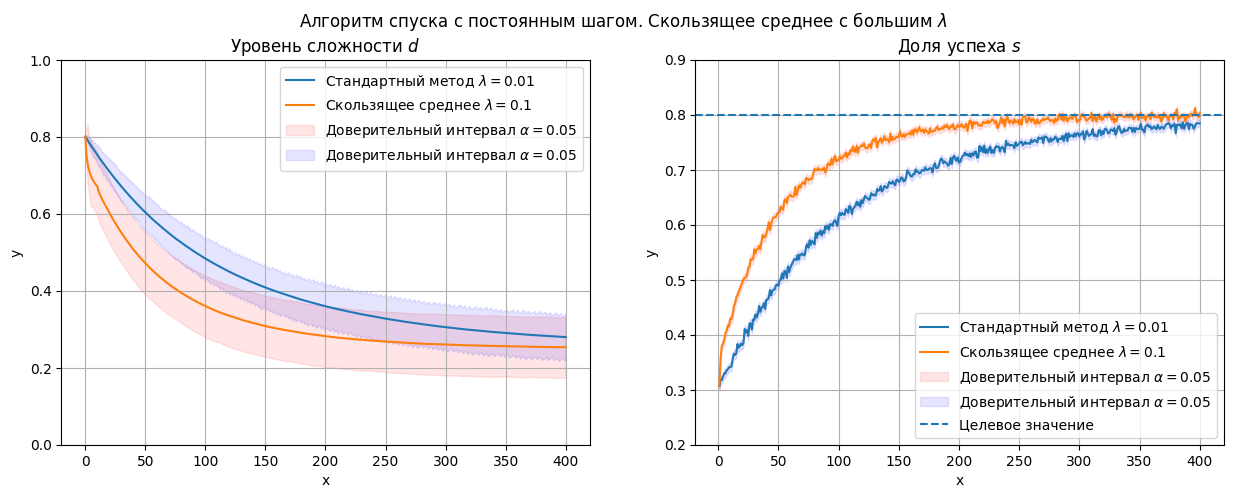
\includegraphics[width=0.9\textwidth]{assets/work/rating/4/lambda_0.01_0.1.png}
    \caption{Метод скользящего среднего позволяет использовать больший параметр шага, не теряя устойчивость метода}
    \label{exp4:better_stability}
\end{figure}
\begin{figure}[h]
    \centering
    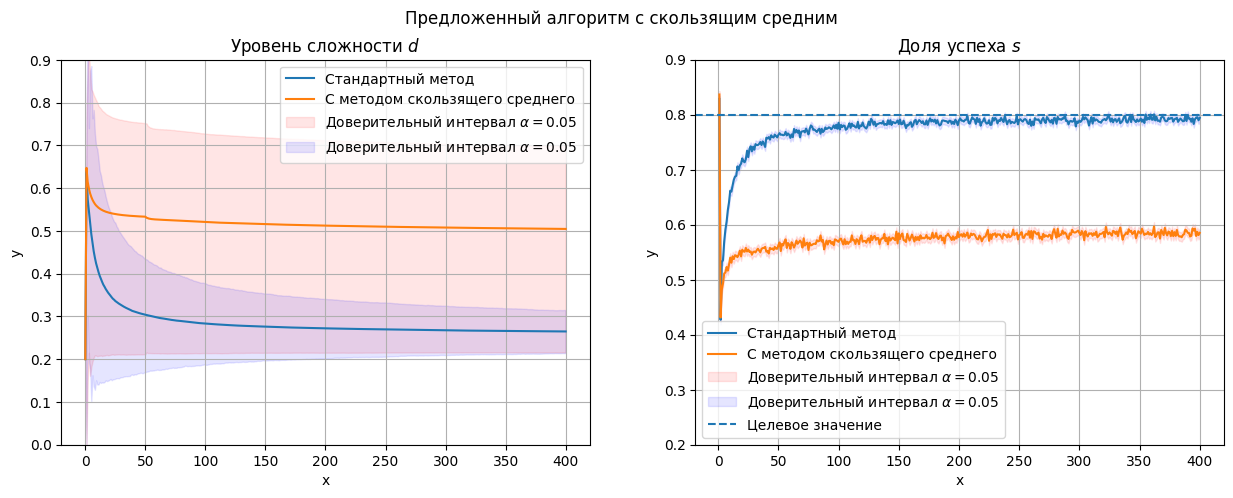
\includegraphics[width=0.9\textwidth]{assets/work/rating/4/adaptive.png}
    \caption{Метод скользящего среднего не применим к предложенному алгоритму}
    \label{exp4:not_applied}
\end{figure}
\begin{table}
    \centering
    \begin{tabular}{ ||c | c|| }
        \hline
        \text{Название алгоритма} &  \text{Число шагов}\\
        \hline 
        \text{Алгоритм Р.-М. со скользящим средним $\lambda=0.01$} & \text{Не сошелся} \\
        \text{Алгоритм Р.-М. со скользящим средним $\lambda=0.1$} & $250\pm 40$  \\
        \text{Адаптированный алгоритм  Р.-М. со скользящим средним } & \text{Не сошелся}\\
        \hline 
    \end{tabular}
    \caption{Сравнение числа шагов с применением метода скользящего среднего}
    \label{exp4:table}
\end{table}

Расходимость предложенного метода связана с нарушениями условий \ref{polyak_assumptions}.

Таким образом, метод скользящего среднего \begin{enumerate}
    \item позволяет использовать больший шаг для обеспечения большей скорости сходимости
    \item не применим к предложенному алгоритму
\end{enumerate}

Полный набор задач моделирования приведен в аппендиксе работы \ref{numeric_modeling}.